\documentclass[logo,reportComp]{thesis}
\usepackage[cpp,pseudo]{mypackage}

\title{计算机图形学}
\subtitle{作业一:SIGGRAPH学术专题整理}
\school{数据科学与计算机学院}
\author{陈鸿峥}
\classname{17大数据与人工智能}
\stunum{17341015}
\headercontext{计算机图形学作业}
\lstset{language=python}

\begin{document}

\maketitle

本文将对SIGGRAPH 2019~\cite{siggraph,siggraph_tech}中的三个专题部分进行介绍与总结,包括神经网络渲染(第\ref{sec:rendering}节)、视野综合(第\ref{sec:view}节)及动作控制(第\ref{sec:motion}节)。

\section{神经网络渲染(Neural Rendering)}
\label{sec:rendering}
渲染(rendering)作为计算机图形学里一个重要的组成部分,决定了图像最终呈现在我们眼前的样子。
如老师上课所介绍的,渲染包括从3D模型中生成2D影像、真实感渲染和非真实感渲染等。
而本次SIGGRAPH'19本主题的几篇文章都侧重于真实感渲染。

在上个世纪80年代,David Immel和James Kajiya就已经提出了渲染方程\cite{rendering_equ},
\[L_{{{\text{o}}}}({\mathbf  x},\,\omega _{{{\text{o}}}},\,\lambda ,\,t)\,=\,L_{e}({\mathbf  x},\,\omega _{{{\text{o}}}},\,\lambda ,\,t)\ +\,\int _{\Omega }f_{r}({\mathbf  x},\,\omega _{{{\text{i}}}},\,\omega _{{{\text{o}}}},\,\lambda ,\,t)\,L_{{{\text{i}}}}({\mathbf  x},\,\omega _{{{\text{i}}}},\,\lambda ,\,t)\,(\omega _{{{\text{i}}}}\,\cdot \,{\mathbf  n})\,\operatorname d\omega _{{{\text{i}}}}\]
它阐明了从一个点$x$沿着特定的观察方向所发出的光的大小,从而奠定了渲染的整体框架。

而随着计算机硬件的发展,快速求解上面的方程并不是什么难事。
像Nvidia RTX 2080甚至添加了实时光线追踪功能,更加使得实时渲染变得触手可及。
因而现在关于渲染的研究,已经与早些年的研究方向产生了很大差别。

随着近年来深度学习的发展,CG也开始大量使用神经网络实现一些原有方法难以实现的技术。
其中一个标志性成果是2014年Ian Goodfellow提出的对抗生成网络(Generative Adversarial Networks, GANs)\cite{gan:goodfellow},它能够进行无监督学习,通过生成器和判别器的两者互博,从样本图像中学习特征,并用以生成新的图像。
这也催生出本届SIGGRAPH的这一个主题,即利用神经网络生成尽可能真实的虚伪图像。

我浏览了该主题下的五篇文章,他们无一例外使用GAN进行图像的生成。
\begin{itemize}
    \item Deferred Neural Rendering\cite{thies:deferred}:输入图像是不清晰的、不完美的,但通过该文提出的方法,可以对图像进行还原,甚至进行复制、剪裁、修改。
\begin{figure}[H]
\centering
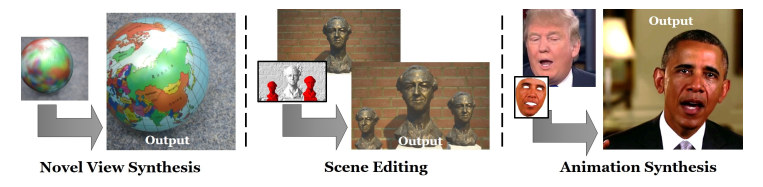
\includegraphics[width=0.8\linewidth]{deferred-neural-rendering.png}
\end{figure}
    \item Neural Reenactment\cite{liu:reenactment}:输入一组动作,可以将对应的动作映射到生成的人。
\begin{figure}[H]
\centering
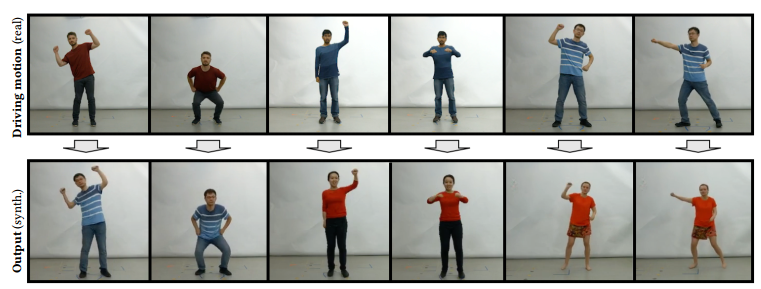
\includegraphics[width=0.8\linewidth]{neural-rendering-and-reenactment.png}
\end{figure}
    \item Neural Volumes\cite{lombardi:volumes}:只需输入不同角度的几张2D图像,就可以还原出整个3D图像。
\begin{figure}[H]
\centering
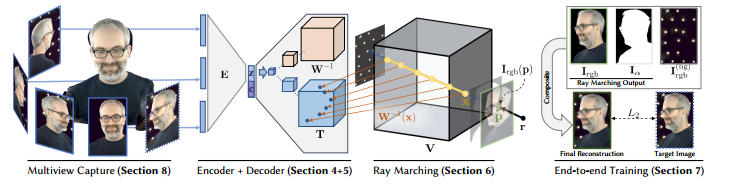
\includegraphics[width=0.8\linewidth]{neural-volumes.png}
\end{figure}
    \item Text-based Editing\cite{fried:text}:可以通过直接增添、删减、修改文本,生成修改后的音频。
\begin{figure}[H]
\centering
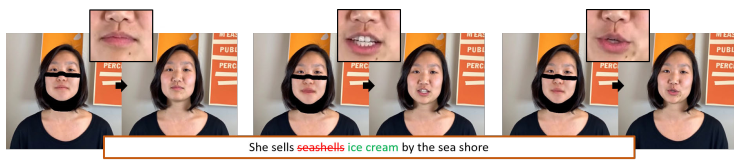
\includegraphics[width=0.8\linewidth]{text-based.png}
\end{figure}
    \item VR Facial Animation\cite{wei:vr}:同样输入几个方向的不同2D图像,可以在VR影像中生成对应的3D真实人物及表情。
\begin{figure}[H]
\centering
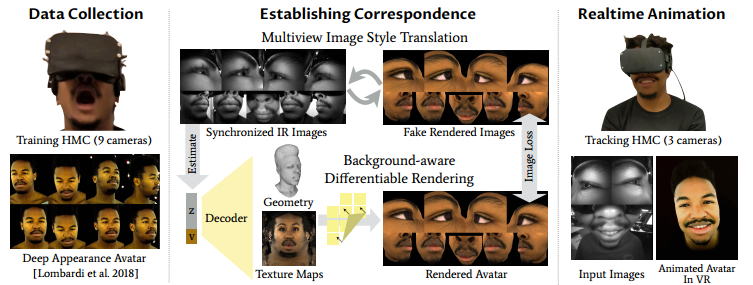
\includegraphics[width=0.8\linewidth]{vr.png}
\end{figure}
\end{itemize}

这一部分的研究在人工智能、计算机视觉方向也是非常热门。
从上面的例子中也可以看出,现在关于图像方面的图形学的研究已经被深度学习侵占了,几乎没有研究还继续采用传统的方法(这从下一个专题中更加能看出来)。
但深度学习确实给图形学带来了很多新的观点,同时也能实现很多以前所做不到的东西。

\section{灯光重制与视图合成(Relighting and View Synthesis)}
\label{sec:view}
这一部分其实也属于真实感渲染的范畴,主要侧重于\textbf{不同光照条件(lighting)和不同角度(viewpoint)的场景重现}。

早在上个世纪90年代,就已经有了视图合成的一些尝试,但是那时需要稠密大量(dense)的输入图片,才可以还原出各个角度的图像。
而现在一个很重要的研究方向则通过于稀疏少量(sparse)的输入图片,还原出完整的全方位图像,以最大程度减少获取(acquisition)图片的成本。

本部分的论文包括下列内容。
\begin{itemize}
	\item Deep View Synthesis\cite{xu:deep_view}:同样输入不同角度(六边形六个角)的图片,合成其他角度的图像,同时可以改变不同的光照。
\begin{figure}[H]
\centering
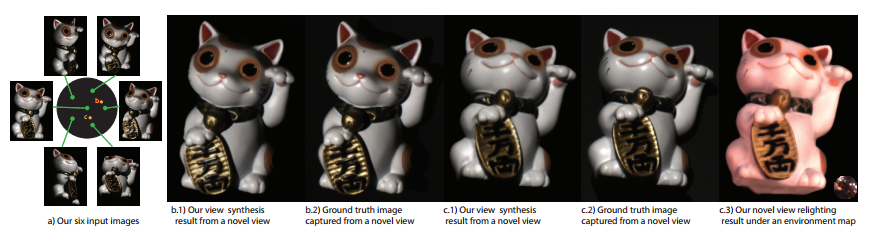
\includegraphics[width=0.8\linewidth]{view-synthesis.png}
\end{figure}
	\item Image Portrait Relighting\cite{sun:image_protrait}:输入人物肖像(手机拍摄即可)及期望的背景照明,输出对应光照条件下的人物肖像
\begin{figure}[H]
\centering
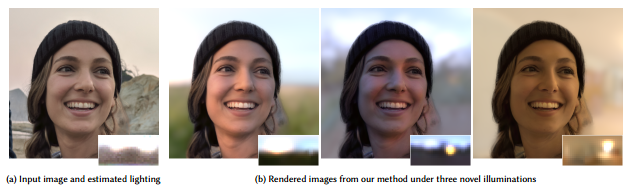
\includegraphics[width=0.8\linewidth]{image-portrait-relighting.png}
\end{figure}
	\item Deep Reflectance Fields\cite{meka:deep_reflectance}:输入同一人像的两张观测图像,还原该人像的光照条件
\begin{figure}[H]
\centering
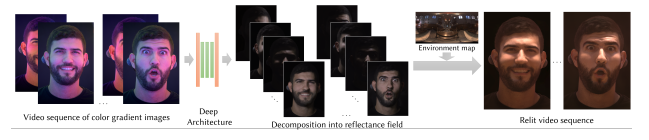
\includegraphics[width=0.8\linewidth]{deep-reflectance.png}
\end{figure}
	\item Multi-view Relighting\cite{philip:multi_view}:输入一张风景图,同样可以方便地改变不同光照条件,生成不同光照下的图像(对应的阴影也能正确生成)
\begin{figure}[H]
\centering
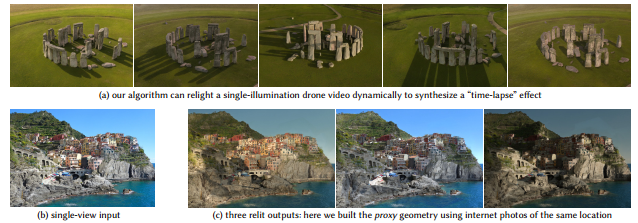
\includegraphics[width=0.8\linewidth]{multi-view-relighting.png}
\end{figure}
\end{itemize}

实际上这部分内容可以看作是一个\textbf{图像翻译}(image-to-image translation)的任务,即输入一张图片以及一些辅助信息,输出一张我们期望得到的图片。
可数学化地表示成
\[\hat{I}_\text{target},\hat{A}_\text{source}=\phi(I_\text{source},A_\text{target})\]
输入原始图片$I_\text{source}$及目标图片的辅助信息$A_\text{target}$,经过复杂的函数变换$\phi$之后,得到新的图片$I_\text{target}$和原始图片的辅助信息$\hat{A}_\text{source}$(后一部分不一定要输出)。
而辅助信息可以是背景光照(第2篇)、摄像机/光源角度信息(第1、4篇)、颜色梯度图(第3篇)等等。

而图像翻译在近几年已经有了很大的突破,首先是2015年Ronneberger提出的U-Net\cite{ronneberger:unet}。
尽管一开始U-Net使用在图像分割上,但后来人们发现将其运用到图像翻译任务上也能取到很好的效果,于是便有了2017年Isola提出的Pix2Pix\cite{isola:pix2pix}。
再到现在,几乎所有图像翻译的任务都会采用U-Net的变体。
如本主题的四篇文章,有三篇都使用了U-Net类似的架构,剩下一篇则使用了传统的CNN(ResNet\cite{he:resnet})架构。

而这种图像翻译任务又与传统的文本翻译有着很大的相通之处,故结合文本翻译中常用的编码-解码模型(encoder-decoder)\cite{sutskever:seq2seq},就能取得很好的效果。
\begin{figure}[H]
\centering
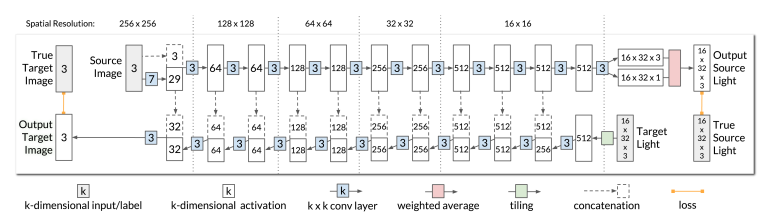
\includegraphics[width=0.8\linewidth]{pr-net.png}
\end{figure}
比如我个人感觉最为逼真酷炫的第二篇论文,就是仿造U-Net设计出如上图这种编码解码结构。
将源图片通过编码器后生成源光照条件,作为中间表示,然后再将目标光照条件输入解码器反向即可生成对应的图像。
这种网络架构的设计是十分自然、合理而且精妙的,这在第三篇论文中也有出现,足以见得其强大之处——少量的图片信息输入,就可以创造出极其逼真的新的图像。

\bigskip

另一方面涉及到的内容是\textbf{基于图像的灯光重制}(Image-Based Relighting)。
这也是计算机图形学中一个重要的研究方向,即在不改变图片内容的情况下,改变图片的光照条件,从而生成新的图片。
这看上去不是什么困难的问题,但要做得好是非常困难的,需要考虑到图片中的大量细节以及不同环境之间的差异。
特别对于人像处理尤为复杂,因为人脸的轮廓是高低起伏而不是平整的,同时人类还有各式各样的表情,可能会戴帽子、戴眼镜等等,涉及头发的处理、人物侧脸的处理等都使得灯光重制极为困难。
如第二第三篇文章都是针对于人物肖像的处理。
而最后一篇文章则针对于大场景的处理,这里的挑战在于光源可能在很远的地方,同时建筑物之间的复杂关系使得阴影的位置、大小、形状等等都会非常复杂,故该文采用了多个神经网络进行处理,其中专门有一个神经网络来对阴影进行估计和生成。

\section{动作控制(Motion is in Control)}
\label{sec:motion}
这一部分与前两部分则有很大的区别,动作控制更偏向于建模(modeling)和动画(animation),其目标就是让计算机模拟更加符合现实生活情况或是让机器人的动作更加能够符合我们的预期。
动作控制对于物理建模的要求非常高,涉及到对复杂的物理过程的模拟,所以会使用到的数学工具也较为高阶,包括微分方程、矩阵分析、最优化理论等。

本部分的几篇论文包含了以下内容。
第二第三篇文章是构建真实的机器人,在机器人上进行操作;而第一第四篇文章则是直接在计算机里构建模型进行模拟。
\begin{itemize}
	\item Interactive Animation Control\cite{ciccone:interative_animation}:可以通过操控骨骼控制点来实现完整的人物动作动画
\begin{figure}[H]
\centering
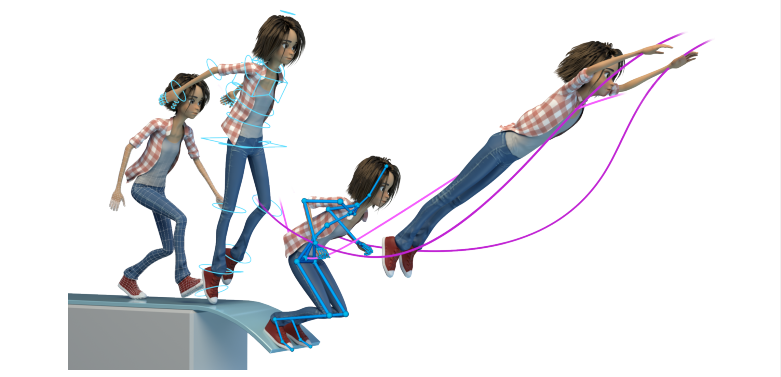
\includegraphics[width=0.8\linewidth]{animation-control.png}
\end{figure}
	\item Robotic Characters\cite{hoshiyari:robotic}:将人体动作映射到对应的机器人模型上,尽可能减少震动带来的影响
\begin{figure}[H]
\centering
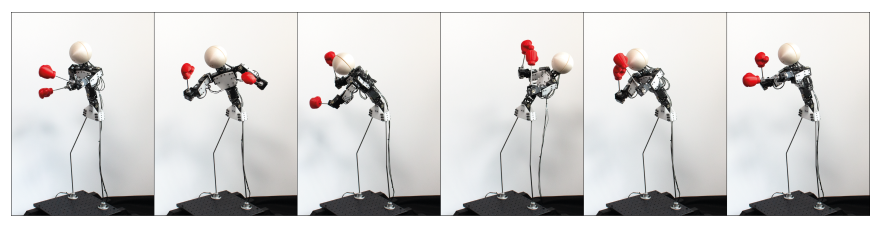
\includegraphics[width=0.8\linewidth]{robotic-character.png}
\end{figure}
	\item PuppetMaster\cite{zimmermann:puppetmaster}:利用机器人实现牵线木偶的操纵
\begin{figure}[H]
\centering
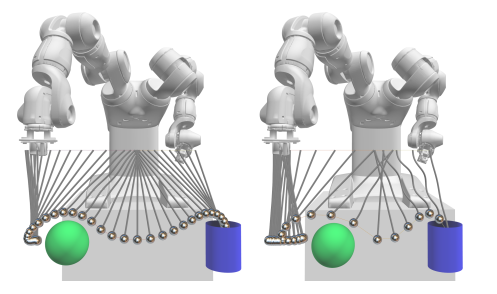
\includegraphics[width=0.4\linewidth]{puppetmaster.png}
\end{figure}
	\item RedMax\cite{wang:redmax}:用于模拟弹性物体的动态物理状况
\begin{figure}[H]
\centering
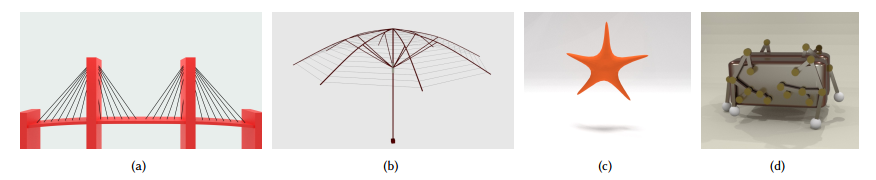
\includegraphics[width=0.8\linewidth]{redmax.png}
\end{figure}
\end{itemize}

在计算机图形学的早期,动画很大程度上依赖于对画家描述的关键帧,通过对这些关键帧进行插值,就可以实现完整的动画。
但是很显然这种方式过为低效,需要大量的人力投入,而且对于物理定律的表现也是非常麻烦的。
因此后来也就诞生了图形学中\textbf{基于物理定律建模}的这个子领域。
最简单的模拟即牛顿第二定律
\[\mathbf {F} =m\,{\frac {\mathrm {d} \mathbf {v} }{\mathrm {d} t}}=m\mathbf {a}\]
通过计算物体的速度、加速度,就可以获得物体运动的轨迹。
但是仅仅模拟牛顿定律,而不添加其他约束显然是不够的,现实生活中的很多现象依然没有办法得到很好的模拟。
因此现在的研究也会侧重于更加细致的动作(如第3篇)以及更加复杂的物理过程(如第2、4篇)的模拟,同时利用数学方法对运动过程做灵敏度分析,并且结合刚体动力学的知识最大程度减少外部因素的影响(如震动)。


\section{总结}
本文主要对SIGGRAPH 2019上的三个主题进行了总结与整理,但囿于本人的学识及时间所限,未能对每一篇论文所采用到的方法或者各个专题再做深入研究。
不过希望在这学期的图形学课程中能够探索自己感兴趣的方向,并做出一些有意思的成果。

\begin{thebibliography}{99}
\bibitem{siggraph} Ke-Sen Huang, SIGGRAPH 2019 papers on the web, \url{http://kesen.realtimerendering.com/sig2019.html}
\bibitem{siggraph_tech} Technical Papers Preview: SIGGRAPH 2019,\url{https://www.youtube.com/watch?v=EhDr3Rs5fTU}
\bibitem{rendering_equ} Wikipedia, Rendering equation, \url{https://en.wikipedia.org/wiki/Rendering_equation}
% 理论计算机图形渲染技术是否已经到了没有什么可以研究的地步了? - 叛逆者的回答 - 知乎
% https://www.zhihu.com/question/29182519/answer/43457554
\bibitem{thies:deferred} Justus Thies, Michael Zollh\"ofer, and Matthias Nie$\beta$ner, \emph{Deferred Neural Rendering: Image Synthesis using Neural Textures}, SIGGRAPH, 2019
\bibitem{liu:reenactment} Lingjie Liu, Weipeng Xu, Michael Zollh\"ofer, Hyeongwoo Kim, Florian Bernard, Marc Habermann, Wenping Wang, and Christian Theobalt, \emph{Neural Rendering and Reenactment of Human Actor Videos}, SIGGRAPH, 2019
\bibitem{lombardi:volumes} Stephen Lombardi, Tomas Simon, Jason Saragih, Gabriel Schwartz, Andreas Lehrmann, and Yaser Sheikh, \emph{Neural Volumes: Learning Dynamic Renderable Volumes from Images}, SIGGRAPH, 2019
\bibitem{fried:text} Ohad Fried, Ayush Tewari, Michael Zollh\"ofer, Adam Finkelstein, Eli Shechtman, Dan B. Goldman, Kyle Genova, Zeyu Jin, Christian Theobalt, and Maneesh Agrawala, \emph{Text-based Editing of Talking-head Video}, SIGGRAPH, 2019
\bibitem{wei:vr} Shih-En Wei, Jason Saragih, Tomas Simon, Adam W. Harley, Stephen Lombardi, Michal Perdoch, Alexander Hypes, Dawei Wang, Hernan Badino, and Yaser Sheikh, \emph{VR Facial Animation via Multiview Image Translation}, SIGGRAPH, 2019
\bibitem{xu:deep_view} Zexiang Xu, Sai Bi, Kalyan Sunkavalli, Sunil Hadap, Hao Su, and Ravi Ramamoorthi, \emph{Deep View Synthesis from Sparse Photometric Images}, SIGGRAPH, 2019
\bibitem{sun:image_protrait} Tiancheng Sun, Jonathan T. Barron, Yun-Ta Tsai, Zexiang Xu, Xueming Yu, Graham Fyffe, Christoph Rhemann, Jay Busch, Paul Debevec, and Ravi Ramamoorthi, \emph{Single Image Portrait Relighting}, SIGGRAPH, 2019
\bibitem{meka:deep_reflectance} Abhimitra Meka, Christian Häne, Rohit Pandey, Michael Zollh\"ofer, Sean Fanello, Graham Fyffe, Adarsh Kowdle, Xueming Yu, Jay Busch, Jason Dourgarian, Peter Denny, Sofen Bouaziz, Peter Lincoln, Matt Whalen, Geoff Harvey, Jonathan Taylor, Shahram Izadi, Andrea Tagliasacchi, Paul Debevec, Christian Theobalt, Julien Valentin, and Christoph Rhemann, \emph{Deep Reflectance Fields: High-Quality Facial Reflectance Field Inference from
Color Gradient Illumination}, SIGGRAPH, 2019
\bibitem{philip:multi_view} Julien Philip, Micha\"el Gharbi, Tinghui Zhou, Alexei A. Efros, and George Drettakis, \emph{Multi-view Relighting using a Geometry-Aware Network}, SIGGRAPH, 2019
\bibitem{ciccone:interative_animation} Lo\"ic Ciccone, Cengiz Öztireli, and Robert W. Sumner, \emph{Tangent-Space Optimization for Interactive Animation Control}, SIGGRAPH, 2019
\bibitem{hoshiyari:robotic} Shayan Hoshyari, Hongyi Xu, Espen Knoop, Stelian Coros, and Moritz
B\"acher, \emph{Vibration-Minimizing Motion Retargeting for Robotic Characters}, SIGGRAPH, 2019
\bibitem{zimmermann:puppetmaster} Simon Zimmermann, Roi Poranne, James M. Bern, and Stelian Coros, \emph{PuppetMaster: Robotic Animation of Marionettes}, SIGGRAPH, 2019
\bibitem{wang:redmax} Ying Wang, Nicholas J. Weidner, Margaret A. Baxter, Yura Hwang, Danny M. Kaufman, and Shinjiro Sueda, \emph{RedMax: Effcient \& Flexible Approach for Articulated Dynamics}, SIGGRAPH, 2019
\bibitem{gan:goodfellow} Ian J. Goodfellow, Jean Pouget-Abadie, Mehdi Mirza, Bing Xu, David Warde-Farley, Sherjil Ozairy, Aaron Courville, and Yoshua Bengio, \emph{Generative Adversarial Nets}, arXiv:1406.2661v1, 2014
\bibitem{he:resnet} Kaiming He, Xiangyu Zhang, Shaoqing Ren, and Jian Sun, \emph{Deep Residual Learning for Image Recognition}, arXiv:1512.03385, 2015
\bibitem{sutskever:seq2seq} Ilya Sutskever, Oriol Vinyals, and Quoc V. Le, \emph{Sequence to Sequence Learning with Neural Networks}, NeurIPS, 2014
\bibitem{ronneberger:unet} Olaf Ronneberger, Philipp Fischer, and Thomas Brox, \emph{U-Net: Convolutional Networks for Biomedical Image Segmentation}, arXiv:1505.04597, 2015
\bibitem{isola:pix2pix} Phillip Isola, Jun-Yan Zhu, Tinghui Zhou, and Alexei A. Efros, \emph{Image-to-Image Translation with Conditional Adversarial Networks}, CVPR, 2017
\end{thebibliography}

% Photo Science -> Semantic Photo Manipulation With a Generative Image Prior

\end{document}

% 参考 2019 年计算机图形学顶级会议 SIGGRAPH 2019(http://kesen.realtimerendering.com/sig2019.html)或 SIGGRAPH Asia 2018(http://kesen.realtimerendering.com/siga2018Papers.htm)上的学术专题和相关论文主页,并从中任意选择3个主题,查阅相关文献和网络资料,陈述这些主题涉及到图形学中的哪些技术(可图文并茂,每个介绍大于 400 字)。

% 说明:
% 作业用电子版 PDF 格式提交, 发送到课程邮箱:
% cgcourse_homework@qq.com,
% 若 2 天内没收到自动回复,请重新发邮件。 请于 9 月 7 日前提交。

% PDF 文件名格式如下:
% 班级 + 学号 + 姓名 + HW1
% 例: 17 计科+17000001+张三+HW1